% ----- CHAPTER 6: REMARKS AND FUTURE WORK ----- %

This dissertation pulls in results from a number of disparate topics related to elliptic curves, with the general approach being ``do enough to establish results that are sufficient to support the main theorems, then move on". As such, many of the bounds and statements obtained of the course of this work are very far from optimal, and the ultimate running time of, say, Algorithm \ref{algo:compute_rank} could be considerably improved if these bounds were tightened. Beyond this there are natural generalizations to the results in this work that should be considered, We list below the areas where results could be improved upon or generalized, and in so doing detail directions for possible future work.

%%%%%%%%%%%%%%%%%%%%%%%%%%%%%%%%%%%%%%%%%%%%%%%%%%%%%%%
\subsection{Implementing and optimizing the rank algorithm}

I coded up a na\"{i}ve implementation of Algorithm \ref{algo:compute_rank} in Sage to collect supporting data for inclusion in this dissertation, but the algorithm is calling out for a dedicated optimized implementation for general use. Much of the hard work has already been done -- for example, Bradshaw provided a Sage implementation of provable motivic $L$-function evaluation in \cite{Bra-2010}, and Sage already includes functionality to compute the real period of an elliptic curve. \\

There are several optimizations that should be included in any implementation. Three which immediately spring to mind are as follows:
\begin{itemize}
\item One should check for torsion on $E$, which is quick to do. Doing so results in up to 16 less bits of precision needed when evaluating $L_E(s)$.
\item It might be advantageous to compute the Tamagawa product $\prod_p c_p$ if it can be quickly done. Again, this results in a larger lower bound on the leading Taylor coefficient of $C_E$, and thus less precision needed when evaluating $L_E(s)$.
\item The $r_{an}(E) < a\log N_E + b$ bounds used for analytic rank are in practice far too crude; in reality the vast majority of curves (if you believe the folklore conjecture, asymptotically 100\%) have rank 0 or 1, and maximum observed rank goes more like $\sqrt{\log N_E}$. It therefore makes sense to obtain a better upper bound on the rank of a given curve up front; this then gives a better lower bound on the regulator and thus further reduces the required precision when provably evaluating $L_E(s)$. One could, for example, run the $\sinc^2$ sum algorithm exhibited in Section \ref{sec:sinc_squared_sum} with some small choice of $\Delta$, which doesn't require direct evaluation of $L_E(s)$.
\end{itemize}

%%%%%%%%%%%%%%%%%%%%%%%%%%%%%%%%%%%%%%%%%%%%%%%%%%%%%%%
\subsection{Generalizing results to modular $L$-functions of arbitrary weight and level}

The results in this thesis revolve around working with the $L$-function attached to a given elliptic curve. By the modularity theorem \cite{BCDT-2011}, each of these is actually the $L$-function attached to a certain weight 2 integral cuspidal eigenform of level $N_E$, where $N_E$ is the conductor of the curve in question. \\

In general we can attach an $L$-function to a cuspidal eigenform of arbitrary weight and level. Many of the results in this dissertation should carry over naturally, allowing us address the issue of computing the analytic rank of higher-weight modular $L$-functions. Specifically, given an analogue of BSD we should be able to show that an algorithm exists to compute the analytic rank of a modular $L$-function that is polynomial-time in the level of that form. An immediate question would then be: how does such a method scale with the {\it weight} of the form? \\

Moreover, the $\sinc^2$ zero sum method to bound analytic rank from above should transfer directly to higher weight forms. We hope in future to extend the functionality of the Sage code to accommodate for this -- in fact, the code layout was designed with this extensibility explicitly in mind.

%%%%%%%%%%%%%%%%%%%%%%%%%%%%%%%%%%%%%%%%%%%%%%%%%%%%%%%
\subsection{CM curves and families of quadratic twists}

Two related questions that we can ask are:
\begin{itemize}
\item Can we get better bounds and results if we restrict ourselves to considering CM curves?
\item Do there exist optimizations for Algorithm \ref{algo:compute_rank} and other results if we consider the family of quadratic twists of a given elliptic curve? How does complexity scale with the twisting parameter $d$?
\end{itemize}

In both cases, we should ask the question: how do the BSD invariants (especially the regulator and real period) vary within a given family? At the very least the real periods within a family of twists is very rigidly controlled, so we should for be able to write down the required precision in Algorithm \ref{algo:compute_rank} as a function of conductor without needing to compute the real period for each curve. \\

Some work has already gone into considering the case of quadratic twists of a given curve -- see \cite{DeRo-2007}. It would be interesting to see if these ideas could be incorporated to improve the results in this thesis.

%%%%%%%%%%%%%%%%%%%%%%%%%%%%%%%%%%%%%%%%%%%%%%%%%%%%%%%
\subsection{Bounding analytic rank from above in terms of conductor}

To establish a lower bound on the regulator of an elliptic curve in terms of its conductor we require an upper bound on the analytic rank. To this end we invoke Corollaries \ref{cor:logderiv_rank_bound} and \ref{cor:better_an_bound}, stating that maximum analytic rank is bounded by a constant times $\log N_E$ plus another explicit constant. \\

However, Corollary \ref{cor:rank_slower_than_log_N} asserts that, contingent on GRH, maximum analytic rank of in fact grows slower than any multiple of $\log N_E$. We would like to use this result more effectively, but the issue lies in making the constant $K_\epsilon$ explicit in terms of the $\epsilon$ chosen. This translates to bounding the $c_n$ sum
\begin{equation}
\sum_{n < e^{2\pi \Delta}} c_n \cdot \left(1-\frac{\log n}{2\pi \Delta}\right)
\end{equation}
in terms of the parameter $\Delta$. \\

A natural question we can ask, and hopefully answer, is ``can this be done effectively"? Empirically, the $c_n$ sum is seldom more than a handful of units in magnitude; however, the fact that the sum is carried out over prime powers and large amounts of cancellation due to the changing signs of the $c_n$ coefficients means that this term is tricky to control [note that one can readily obtain a naive explicit bound that is exponential in $\log \Delta$, but this is of limited practical use]. \\

Nevertheless, if one could show that the sum grows at most polynomial in $\log \Delta$ (regardless of $E$) and obtain explicit constants, then we should be able to show that the lower bound on the regulator of $E$ would go to zero more slowly than any negative power of $N$, as appears to be the case in practice. \\

%%%%%%%%%%%%%%%%%%%%%%%%%%%%%%%%%%%%%%%%%%%%%%%%%%%%%%%
\subsection{The regulator}

The lower bound on $\Reg_E$ could potentially be improved in multiple ways. Firstly, the result relies on the Hindry-Silverman/Elkies' result \cite{Elk-2006} that, contingent on ABC, for any rational point $P$ on curve $E$ with discriminant $D_E$ obeys
\begin{equation}
\hat{h}(P) > M_0 \log(D_E),
\end{equation}
where $M_E \ge 3.94\times 10^{-5}$. This result is in all probability not optimal. An improvement in the lower bound on point height would result in a direct improvement on the constants involved in the lower bound on the regulator, and thus the precision required in the evaluation of $L_E(s)$ in Algorithm \ref{algo:compute_rank}. Again, this is a deep topic, so new insight here won't come easily. \\

What is perhaps a bit more tractable is to continue in the same vein as in the beginning of the proof of Theorem \ref{thm:regulator_lower_bound}: artificially increase the size of the constant, and check computationally that it holds for all curves up to a given conductor bound. We chose a bound of $N=350000$ simply because that is where Cremona's tables currently go to, but there is no theoretical reason one has to stop there. This option of course pays the price of being computationally much more tedious. \\

Finally, the lower bound on $\Reg_E$ contains a reciprocal Gamma factor, which means that the lower bound decays faster than any power of $\log N_E$. This factor arises from the lower bound on the minimum covolume of a lattice in $\RR^r$ with a fixed minimum vector length (Lemma \ref{lem:covolume_lower_bound}), which is most likely not optimal. If a better lower bound could be exhibited on Lattice covolume as a function of dimension, it is conceivable that we could eliminate the Gamma factor entirely. This is desirable, as we would then have that $\Reg_E$ is bounded below by a negative power of the conductor.

%%%%%%%%%%%%%%%%%%%%%%%%%%%%%%%%%%%%%%%%%%%%%%%%%%%%%%%
\subsubsection{The real period}

The lower bound on the real period of an elliptic curve could potentially be improved further. Specifically, in  we would like to make the constant in Theorem \ref{thm:real_period_lower_bound} completely explicit as a function of $\epsilon$, which would remove the need to compute $\Omega_E$ in order to determine the precision. \\

Secondly, the bound of $\Reg_E > K_{\epsilon}\cdot (N_E)^{-1.5-\epsilon}$ does not seem to be very tight; empirically it would appear that minimum real period goes more like $(N_E)^{-1}$. It would be useful to see if the proofs in Section \ref{sec:real_period} could be reworked to make the results conform more closely with the observed data.


%We invoke ABC and Szpiro's Conjecture when proving lower bounds on the real period in terms of the conductor; however, this isn't strictly necessary. Since the minimal discriminant of a rational elliptic curve is $12$th-power free (outside of $2$ and $3$), there is a natural power bound of the minimal discriminant in terms of the conductor:
%\begin{equation}
%|D_E| \le K\cdot \left(N_E\right)^{12},
%\end{equation}
%where $K$ is an explicit constant that accounts for the potentially higher powers of $2$ and $3$ (which can and should be easily made explicit). As such, we should be able to completely remove the dependence on Szpiro in Theorem \ref{thm:real_period_lower_bound}, at the expense of having less optimal constants. \\
%
%Note that this line was deliberately not pursued in this dissertation, as the assumption of ABC is required for bounds on the regulator in any case. However, ultimately we would like to remove reliance on ABC (if possible) entirely; bounds on the real period are not the obstruction when it comes to this.

%%%%%%%%%%%%%%%%%%%%%%%%%%%%%%%%%%%%%%%%%%%%%%%%%%%%%%%
\subsection{Convergence rate and and convexity statements on the sinc$^2$ rank bounding sum}

Equation \ref{eqn:sincsquared_sum} gives the analytic rank of $E$ as a limit:
\begin{align}
r_E = \quad & \lim_{\Delta \to \infty} \;\; \frac{1}{\Delta \pi}\left[\left(-\eta + \log\left(\frac{\sqrt{N}}{2\pi}\right)\right)+ \frac{1}{2\pi \Delta}\left(\frac{\pi^2}{6} - \Li_2\left(e^{-2\pi \Delta}\right)\right)  \right. \nonumber \\
&+ \left.\sum_{n<e^{2\pi \Delta}} c_n \cdot \left(1-\frac{\log n}{2\pi \Delta}\right)\right].
\end{align}

\begin{figure}[!h]
    \centering
    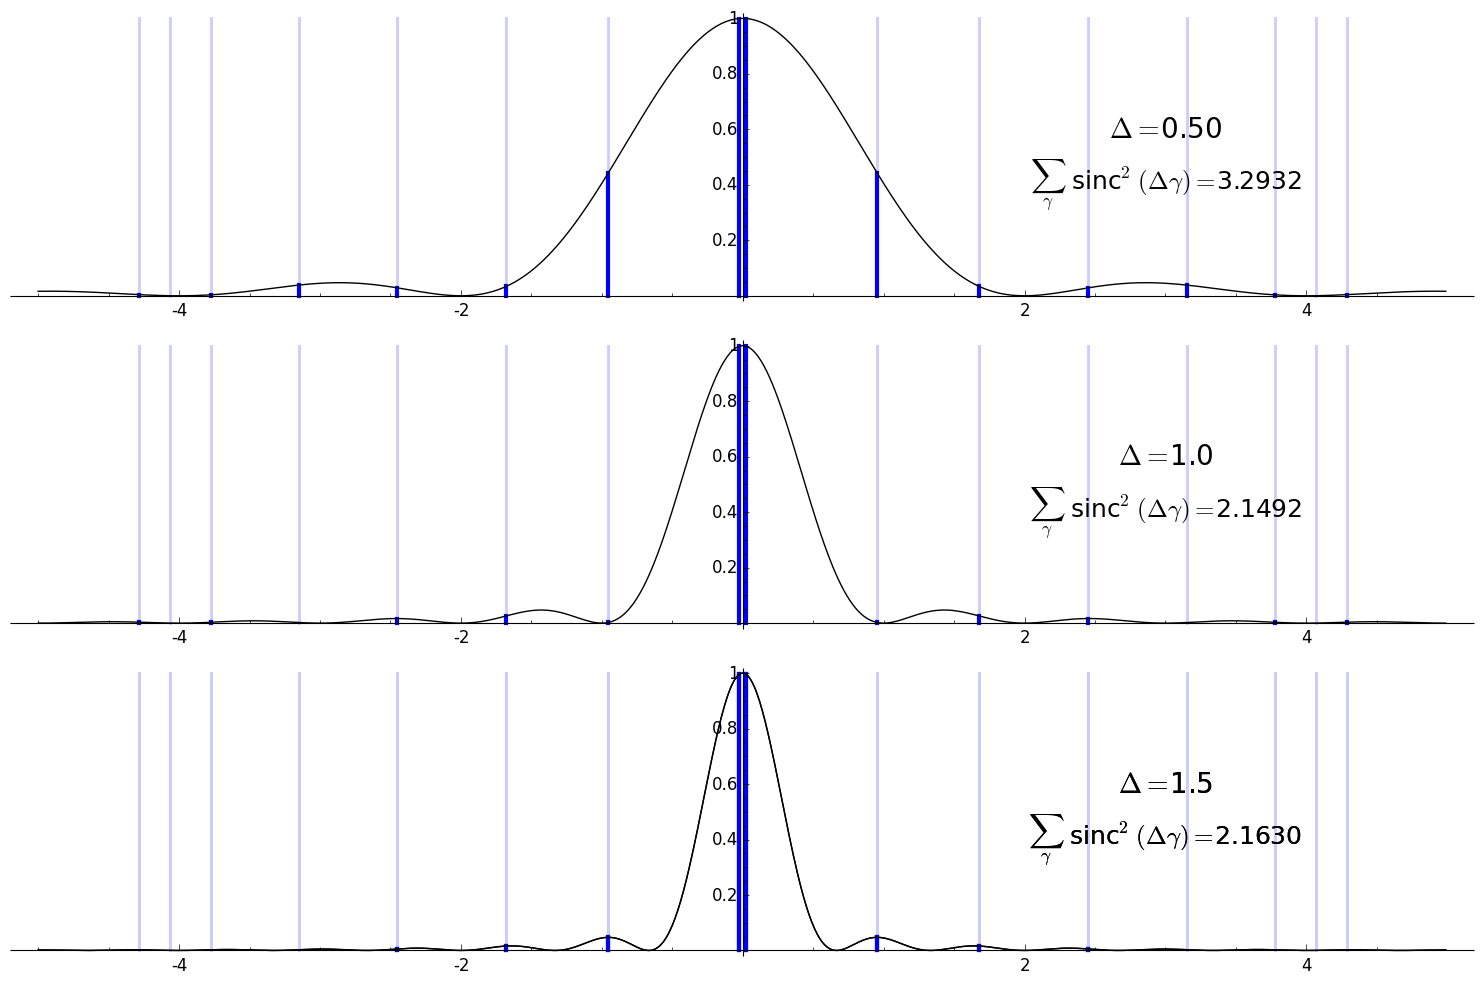
\includegraphics[width=1.0\textwidth]{graphics/256944c1_zero_sum.png}
    \caption{A graphic representation of the $\sinc^2$ sum for the Cremona curve {\tt 256944c1} , a rank 0 curve with conductor $N_E=256944$, for $\Delta = 0.5$, $1.0$ and $1.5$.}
    \label{fig:256944c1_zero_sum}
\end{figure}

However, more work needs to be done regarding the rate of convergence of this sum. We give a result regarding convergence rate of the $\sinc^2$ sum in terms of the bite $\beta_E$ of a curve in Theorem \ref{thm:sinc_squared_sum_with_bite}. However, this is more of a step sideways, as the bite remains a mysterious quantity in its own right. \\

Consider the example in Figure \ref{fig:256944c1_zero_sum}: the Cremona curve {\tt 256944c1}, a rank 0 curve, has a pathologically low-lying zero at $\gamma_0 = 0.02560\ldots$. For small values of $\Delta$, it therefore appears that this curve has analytic rank 2, not zero. In fact, only for $\Delta>\sim 2.815$ does the sum evaluate to a value less than 2 (which, after invoking parity, gives us that it is rank 0). This highlights the fact that some curves -- specifically those with low-lying zeros -- require $\Delta$ to be large for the sum to be within, say, 2 of the true rank of the curve. \\

Furthermore, Figure \ref{fig:256944c1_zero_sum} shows that the convergence from above is unfortunately {\it not} even necessarily monotone: as $\Delta$ is increased the small outlying bumps of the sinc$^2$ function can travel over zeros and temporarily increase the value of the sum. \\

Even though this is the case, we should be able to make some sort of a convexity statement regarding the convergence of the sinc$^2$ sum. This should allow us to use point estimates in the rank estimation code to decide which $\Delta$ values to use on a given curve, and in so doing make the code more efficient. This has the potential to significantly increase the effectiveness of the rank estimation code.

%%%%%%%%%%%%%%%%%%%%%%%%%%%%%%%%%%%%%%%%%%%%%%%%%%%%%%%
\subsection{Better bounds on the bite}

Section \ref{sec:bite} discusses at the topic of the bite of an elliptic curve, namely the quantity
\begin{equation}
\beta_E = \sum_{\gamma \ne 0} \frac{1}{\gamma^2}.
\end{equation}

It would be useful to have better bounds in either direction for this quantity. In terms of bounding from below, we are reasonably confident that the constant $K_{\epsilon}$ in Equation \ref{eqn:bite_lower_bound} can be made explicit in terms of $\epsilon$, given more diligent controlling of the various zero sum-based inequalities. Better yet, it would seem that the bite must grow faster than any multiple of $\log N_E$, and we would like to show that this is the case. It is conceivable that this could also be achieved using the methods detailed in this work. \\

On the other hand, placing an upper bound on the bite is equivalent to bounding the lowest noncentral zero away from the central point. This is a much deeper and more difficult endeavour, equivalent to placing a lower bound on the leading central Taylor coefficient of $\Les$. The latter is done in Chapter \ref{chap:main_theorem}, and in fact a direct corollary of this is that the lowest noncentral zero $\gamma_0$ is bounded below by $(N_E)^{-\alpha}$ for some $\alpha>0$. However, in the leading Taylor coefficient bound a constant introduced from the bound on the real period is never made explicit; while this is good enough to get a polynomial-time rank algorithm out, it {\it isn't} good enough to make the lower bound on $\gamma_0$ explicit. Again, we hope that this issue can be resolved in future work, perhaps by making all constants in bounds on the real period completely explicit.


